\begin{multicols}{3}[\section{Laserlink}]

\rhead{Yuliya Ukolava}
\lfoot{19.05.2016}

\newrefsegment

\begin{tabular}{p{2,1 cm}p{2.7 cm}}
\textbf{Steckbrief}& \\
\end{tabular}
\rowcolors{1}{\topicolor!20}{}
\begin{tabular}{p{2,1 cm}p{2.7 cm}}
      Einsatz seit & ca. 1960\\
      Wellenlängen & \SI{780}{\nano\metre} bis \SI{900}{\nano\metre}, \SI{1550}{\nano\metre} bis \SI{1600}{\nano\metre}\\
      Datenrate & bis \SI{2,5}{Gbit/s}\\
      Verbreitung & Weltweit\\
      Reichweite & bis \SI{4}{\kilo\metre}\\
      Modulation & WDMA\\
      Sendeleistung (optische Leistung) & \SI{1}{\mega\watt} bis \SI{100}{\mega\watt}\\
      Dämpfung & \SI{20}{\decibel/\kilo\metre}\\
\end{tabular}
\par

\subsection*{Überblick}
Bei optischem Richtfunk, auch optische Freiraum(daten)übertragung, Laserlink oder optische Freiraumkommunikation (englisch \textbf{f}ree-\textbf{s}pace \textbf{o}ptical communication, \textbf{FSO}) genannt, handelt es sich um eine Technik zur Übertragung von in der Regel digitalen Daten mittels Licht. Das Datensignal kann unter anderem Sprache oder Videosignale umfassen.

Im optischen Richtfunk wird häufig mit Laser-Links gearbeitet. Dies sind auf Laserstrahlen basierende Richtfunkstationen. Laser-Links können sehr genau ausgerichtet werden und können vor allem da eingesetzt werden, wo nur eine Sichtverbindung mit minimaler Toleranz zulässig ist. Weiterhin haben Laser-Links, gegenüber Mikrowellen-Richtfunkstationen, den Vorteil, dass ihre Streuung im normalen Umfeld wesentlich geringer ausfällt und sie somit sicherer gegen Spionage sind. Sollten jedoch streuende Partikel, wie Rauch in die Sichtverbindung gelangen, können diese den Link so streuen, dass eine Ableitung der Informationen problemlos möglich ist. Da Laser-Links sehr genau sind, sind sie auch sehr störanfällig, was ihre Ausrichtung betrifft. Schon eine Abweichung von wenigen Minuten(Bogenminuten) kann die Datenübertragung erheblich stören. Darüber hinaus kann eine Unterbrechung des Links durch einen lichtundurchlässigen Stoff stattfinden. ~\cite{Laserlink.1}

\subsection*{Technische Erläuterungen}
Die optischen Richtfunksysteme übertragen Daten durch die freie Atmosphäre. Dabei verwenden sie für die Signalübertragung modulierte Laser-Lichtsignale, die eng gebündelt, geradlinig abgestrahlt werden. Für die Verbindung von Datennetzwerken sind die optischen Richtfunksysteme mit  \textbf{LWL}- (\textbf{L}icht\textbf{w}ellen\textbf{l}eiter-) Schnittstellen ausgerüstet. Der Ausgangspunkt ist, dass die Signale an optischen LWL-Schnittstellen zur Verfügung stehen. Im Prinzip kann die aus dem Sende-LWL austretende modulierte Strahlung direkt über die Sendeoptik, die Atmosphäre und die Empfangs-LWL eingekoppelt werden. In der Regel sind jedoch zum Dämpfungsausgleich sowie zur Wellenlängen- und Querschnittsanpassung optoelektronische Zwischenverstärker erforderlich. Diese Zwischenverstärker haben LWL-Schnittstellen an den Ein- und Ausgängen und sind transparent in einem weiten Bitratenbereich. Alle Signale werden protokollunabhängig und transparent übertragen, ohne jede inhaltliche Veränderung oder Ergänzung. Hierzu ist zu bemerken, dass neuere Systeme auch mit bereits integrierten Ethernet, ATM oder E1/T1/E3/T3 Schnittstellen auf dem Markt erhältlich sind. 

Die optischen Richtfunksysteme bestehen aus zwei gleichen optischen Sende- und Empfangsgeräten, die in gegenseitigem Sichtkontakt montiert werden. Jedes Sende- und Empfangsgerät enthält als Hauptkomponenten einen Lasersender und einen Laserempfänger für die atmosphärische Signalübertragung. Vorhanden sind außerdem alle für den Betrieb erforderlichen elektronischen Schaltungen für Signalmodulation -demodulation, Spannungsversorgung und Überwachungsfunktion, einschließlich der Lichtwellenleiter-Schnittstellen (oder bereits integrierte Network Interfaces). Über die in die Rückwand integrierten LWL-Ports können die optischen Richtfunksysteme direkt in lokale Netze integriert werden. 
Der Lasersender wandelt Signale aus dem LWL-Datensatz in leistungsstarke Lichtsignale um, die durch die frei Atmosphäre zum entfernt installierten Sende- und Empfangsgerät übertragen werden. Die Lichtsignale werden dort vom Laserempfänger aufgenommen und in der originalen Signalform über den LWL-Ausgangsport wieder in das Datennetz eingespeist. Die einzigartige, konstruktive Zusammenfassung von Lasersender und Laserempfänger in einer kompakten Anordnung, garantiert ein Höchstmaß an Witterungsschutz, Zuverlässigkeit und Bedienungskomfort. 

Da die Achsen der Lasersender und Laserempfänger werkseitig präzise in die Geräteachsen justiert werden, ist eine optimale Ausrichtung der atmosphärischen Signalverbindung auf einfachste Weise, mit Hilfe von Zielfernrohren, möglich. Dies erleichtert die präzise Feineinstellung der beiden optischen Richtfunksysteme. 

Der Sender hat die Aufgabe, digitale Datensignale via Sendeoptik zum Empfänger zu übertragen. 

Von den verfügbaren Strahlungsquellen sind es vor allem \textbf{GaAIA}s (\textbf{Ga}llium-\textbf{Al}uminum-\textbf{A}rsenide) Lumineszenz- und Laserdioden, die den Anforderungen nach hohem Wirkungsgrad, hoher Strahldichte und einer Modulationsfähigkeit bis in den GHz-Bereich weitgehend gerecht werden. Mit dem elektrischen Digitalsignal wird entweder die Strahlungsintensität direkt gesteuert, oder es wird ein hochfrequenter Zwischenträger in der Phase oder Frequenz digital moduliert. Die direkte Phasenmodulation der optischen Welle bei Laserdioden ist bei der Ausbreitung durch die Atmosphäre im betrachteten Wellenlängenbereich nicht sinnvoll, da die Kohärenz durch Beeinflussungen in der Atmosphäre zumindest teilweise zerstört wird. 

Mit Lumineszenzdioden wird in einem durch entsprechende Dotierung eng begrenztem Halbleitergebiet eine hohe Strahlungsdichte generiert. Diese Infrarote Punktquelle mit z.B. \SI{100}{\micro\metre} Durchmesser und einer Strahldichte von \SI{10}{\watt/\per\square\centi\metre} wird dann mit der Sendeoptik in die Empfängerebene abgebildet. Der Strahlendivergenzwinkel kann durch Wahl der Brennweite der Sendeoptik in weiten Grenzen variiert werden. Energetisch günstig ist natürlich ein schmaler Winkel, damit möglichst viel von der ausgesendeten Sendestrahlung auf den Empfänger konzentriert wird. Da man jedoch davon ausgehen muss, dass der Aufstellungsort des Senders gewissen Schwankungen ausgesetzt ist, sollten bei Systemen ohne eine aufwendige automatische Strahlnachführung Divergenzwinkel unter \SI{2}{\milli\radian} vermieden werden. LEDs strahlen inkohärent mit einer spektralen Bandbreite, die etwa 3\% der optischen Mittelfrequenz beträgt. 
Mit Laserdioden kann bei verbessertem Wirkungsgrad eine höhere Leistungsdichte erzielt werden. Sie werden deshalb vor allem in Systemen für größere Reichweiten eingesetzt. Ansonsten sind Laser mit hoher Kohärenz eher ungünstig für die optische Richtfunkübertragung, da Auslöscheffekte durch Interferenzen sich nachteilig auf den Störabstand auswirken können. Außerdem treten bei kleinen Strahldurchmessern in Sendernähe Strahlungsdichten auf, die bei direktem Blick in die Sendeoptik Augenschädigungen hervorrufen können. Es sind in diesen Fällen besondere Schutzmaßnahmen vorgeschrieben. 

Der Empfänger bündelt mit seiner Empfangsoptik die Signalstrahlung auf den optoelektronischen Wandler. Es besteht die Forderung, mit einem möglichst hohen Wirkungsgrad die optische Strahlung zu demodulieren und ein elektrisches Empfangssignal mit geringer Bitfehlerhäufigkeit zu erhalten. Als Wandler können in dem ausgewählten Wellenlängenbereich \textbf{Si}(\textbf{Si}lizium)-Fotodioden mit oder ohne innerem Verstärkungseffekt eingesetzt werden. Nach der elektronischen Signalaufbereitung in Regel- und Begrenzverstärkern und einer eventuell erforderlichen Demodulation des Zwischenträgers steht das digitale Signal wieder zur Weiterleitung zur Verfügung. 
Durch die Hintergrundstrahlung (Tageslicht, Licht von Beleuchtungseinrichtungen) wird ein Störsignal im Empfänger erzeugt, das die Grenzempfindlichkeit herabsetzt. Es gibt zwei Wege den Einfluss der Hintergrundstrahlung zu minimieren: 
\begin{itemize}
\item Einsatz eines optischen Bandpassfilters für das Nutzsignal und damit Ausblendung der Hintergrundstrahlung
\item Minimierung des Empfangswinkels durch entsprechende Wahl von Demodulatorfläche und Brennweite
\end{itemize}
Die durch Luftturbulenzen erzeugte Stör-Intensitätsmodulation der Strahlung mit einem Spektrum bis etwa \SI{1}{\kilo\hertz} kann auf der Sendeseite durch einen großen Strahlenquerschnitt und auf der Empfangseite durch eine große Empfangsfläche verringert werden. Die restliche Störmodulation wird durch Filterung des demodulierten elektrischen Signals, eine automatische Verstärkungsregelung und Begrenzung des Digitalsignals weitgehend eliminiert. 
Für den Einsatz eines optischen Richtfunksystems sind zwei Bedingungen zu beachten:
\begin{itemize}
\item direkte Sichtverbindung zwischen den zwei Stationen
\item Luftliniendistanz zwischen den zwei Punkten 
\end{itemize}
~\cite{Laserlink.2}

\subsection*{Einsatz}
Optische Freiraumübertragungssysteme heben ihren Einsatzschwerpunkt bei der LAN- Kopplung, beispielsweise zwischen benachbarten Gebäuden. Ihre Vorteile sind eine schnelle Installationsmöglichkeit mit optischen LWL-Schnittstellen zum Netz sowie hohe Datenübertragungsraten bis zu \SI{622}{Gbit/s}. 
Weiterhin besteht keine Restriktion bezüglich der Frequenzbandnutzung. Eine Anbindung an eine Überwachungseinheit erfolgt in einfachsten Fall mittels einer Schnittstelle an einen PC welcher mit entsprechender Software die Überwachung des Übertragungssystems realisiert. 
\end{multicols}
\newpage
\section*{Historische Entwicklung}
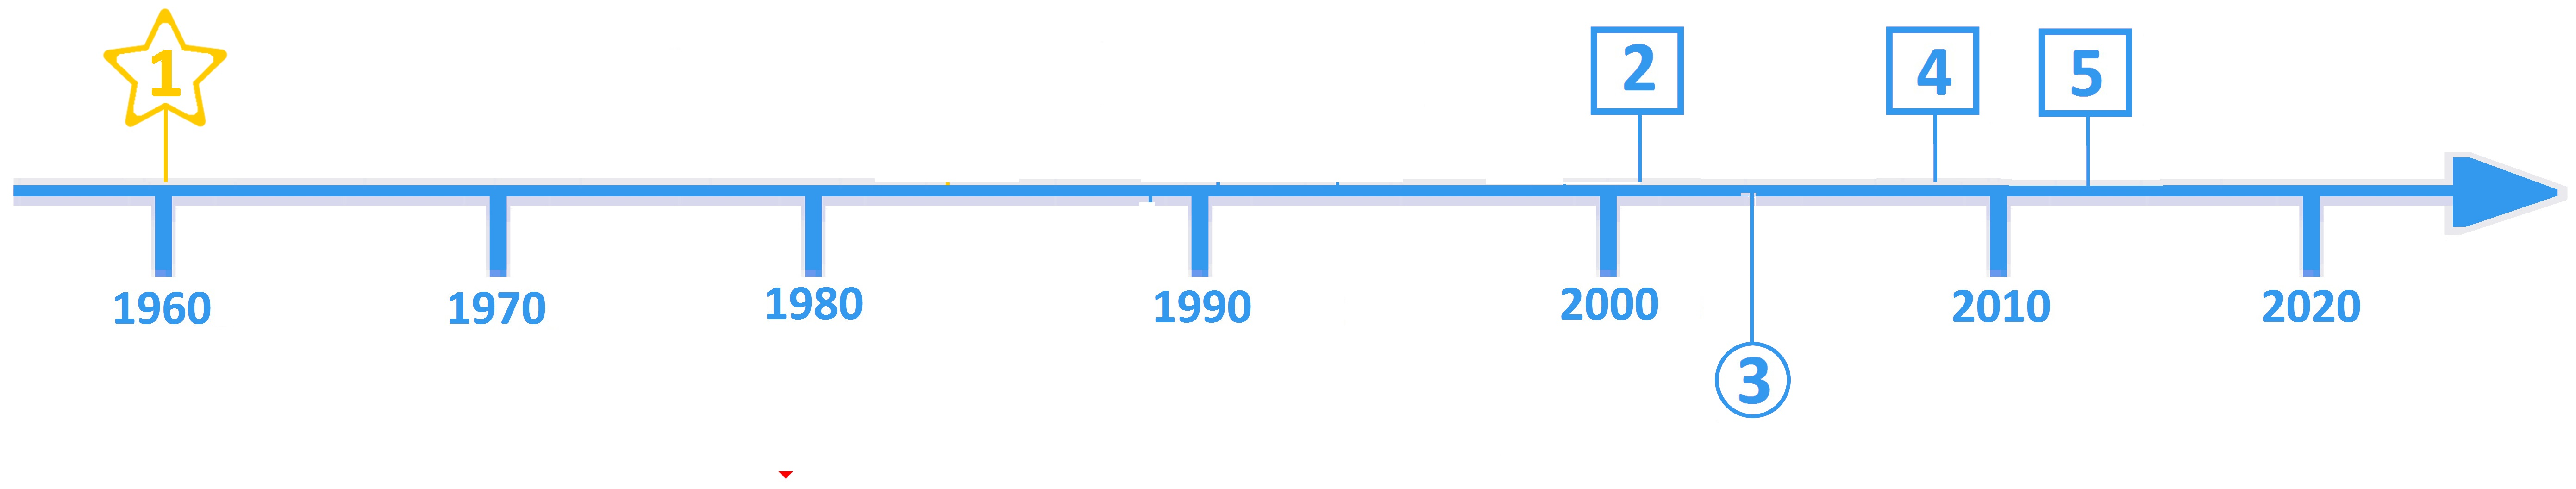
\includegraphics[width=\textwidth]{Kapitel/Laserlink/Grafiken/Zeitstrahl}
\par
\noindent
\rowcolors{2}{}{\topicolor!20}
\begin{tabular}{p{0.5 cm}p{3 cm}p{13.55 cm}}
	Nr. & Datum & Entwicklungsschritte\\
	1 &  1960 & Erfindung des Lasers. ~\cite{Laserlink.5}\\
	2 & 2001 & \textit{Twibright Labs} veröffentlicht eine drahtlose LED-basierte Netzwerkverbindung \textit{Ronja Metropolis}, das erste optische Freiraumsystem mit zurzeit \SI{10}{Mbit/s} in beide Richtungen (Duplex) und max. Reichweite von \SI{1,4}{\kilo\metre}.~\cite{Laserlink.5}\\
	3 & 2004 & \textit{Visible Light Communication Consortium} gegründet in Japan.~\cite{Laserlink.5}\\
	4 & 2008 & MRV Communications führt ein optisches freiraumkommunikation-basiertes System mit einer Datenrate von \SI{10}{GB/s} mit Reichweite von \SI{2}{\kilo\metre}. (Dieses System ist nicht mehr vorhanden; am Ende wurde die Reichweite des Produkts auf \SI{350}{\metre} gesenkt.~\cite{Laserlink.5}\\
	5 &  2013 &  das Unternehmen \textit{MOSTCOM} begann seriell ein neues drahtloses Kommunikationssystem herzustellen, die auch eine Reichweite von bis zu \SI{2,5}{\kilo\metre} mit einer Datenrate von \SI{10}{GB/s} hat, aber eine 99,99\% Betriebszeit zu bekommen, habe die Designer eine Hybrid-Lösung verwendet, d.h. die Datenrate sinkt auf extrem niedrige Werte bei atmosphärischen Störungen.~\cite{Laserlink.5}\\
\end{tabular}
\par
\begin{multicols}{3}
Eine solche Einheit bietet den Anwender die Möglichkeit, jederzeit klare Aussagen über die Streckensicherheit und Stabilität des Systems zu treffen. Besonders bei der Übertragung von Sprachkanälen ist das von Vorteil, während eine solche Überwachung bei einem System in dem TCP/IP unterstützte Daten übertragen werden nicht besonders sinnvoll erscheint. ~\cite{Laserlink.3}
Weitere Anwendungen:
\begin{itemize}
      \item LAN-zu-LAN-Verbindungen auf Betriebsgeländen (Fast Ethernet; Gigabit Ethernet)
      \item LAN-zu-LAN-Verbindungen innerhalb einer Stadt
      \item Überwindung von Verkehrswegen und Hindernissen (zum Beispiel Straßen und Flüssen)
      \item schnell bereitzustellender Breitband-Zugang zu Metronetzen von Telecom-Anbietern (Carriern)
      \item temporärer Netzausbau
      \item Erhöhung der Übertragungssicherheit durch zusätzliche Verbindung mittels FSO (Redundanz)
      \item kombinierte Sprach-Daten-Verbindungen
      \item Einsatz zur Wiederherstellung von zer- bzw. gestörten Verbindungen (Disaster Recovery)
      \item Einsatz zur Verbindung von Netzen und Digipeater im Amateurfunk
      \item Verzicht auf die Anmietung einer Standleitung eines Telekommunikationsanbieters
      \item Kommunikation zwischen Satelliten, sowie Satelliten und Bodenstationen
      \item Industrielles Logistikumfeld: Optische Datenübertragung kann für die Positionsbestimmung innerbetrieblicher Transportsysteme, z. B. flurgebundene Unstetigförderer wie Gabelstapler, eingesetzt werden. Dabei senden lokale Baken mittels LEDs eine Information über ihre Position an eine Empfangseinheit auf dem Flurförderzeug.
\end{itemize} ~\cite{Laserlink.4}
\begin{Figure}
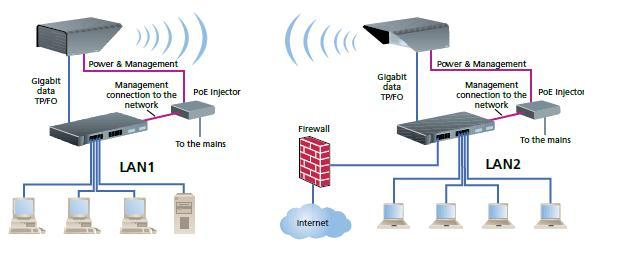
\includegraphics[width=\linewidth]{Kapitel/Laserlink/Grafiken/Laserlink} 
\captionof{figure}{Abb. LAN-zu-LAN-Verbindung~\cite{Laserlink.6}}
\end{Figure}

\subsection*{Ausblick}
Optische Richtfunksysteme werden nach übereinstimmenden Prognosen führender Marktforschungsinstitute in den kommenden Jahren einen weiteren Aufschwung erleben. Wichtige Gründe dafür sind die Flexibilität der Lösungen, ihre geringen Folgekosten und die einfache Installation. Der Ausbau des Serviceangebots und die ständige Weiterentwicklung innovativer Produkte helfen zusätzlich, die Wachstumschancen zu erhöhen. 

Die Einsatzgebiete für Netzwerke und deren drahtlose Verbindung untereinander liegen bei Gebäuden, die nicht oder nur schwer mit Kupfer- bzw. Glasfaserkabeln zu verkoppeln sind. Hauptabnehmer für drahtlose Systeme sind Industrie und Handel. ~\cite{Laserlink.1}
\printbibliography[segment=20,heading=subbibliography]
\end{multicols}
\newpage
